\documentclass[aspectratio=169,10pt]{beamer}

\usepackage[utf8]{inputenc}
\usepackage[T1]{fontenc}
\usepackage{lmodern}
\usepackage{microtype}
\usepackage{amsmath,amssymb}
\usepackage{booktabs}
\usepackage{array}
\usepackage{graphicx}
\usepackage{tikz}
\usetikzlibrary{arrows.meta,positioning,shapes.geometric}
\usepackage{algorithm}
\usepackage{algorithmic}
\usepackage{xcolor}
\usepackage{caption}
\usepackage{subcaption}
\usepackage{ragged2e}

% ─── Theme ───────────────────────────────────────────────────────────────────
\usetheme{Madrid}
\usecolortheme{default}
\setbeamertemplate{navigation symbols}{}
\setbeamersize{text margin left=0.5cm, text margin right=0.5cm}
\setbeamerfont{title}{size=\Large,series=\bfseries}
\setbeamerfont{subtitle}{size=\normalsize}
\setbeamerfont{author}{size=\small}
\setbeamerfont{institute}{size=\small}
\setbeamerfont{date}{size=\small}
\setbeamerfont{frametitle}{size=\normalsize,series=\bfseries}
\setbeamerfont{block title}{size=\small,series=\bfseries}
\setbeamerfont{block body}{size=\footnotesize}

\definecolor{ikm}{RGB}{0,82,147}       % IKM blue
\definecolor{ikmlight}{RGB}{204,221,237}
\definecolor{ikmaccent}{RGB}{0,130,200}
\setbeamercolor{frametitle}{bg=ikm,fg=white}
\setbeamercolor{title}{fg=ikm}
\setbeamercolor{block title}{bg=ikm,fg=white}
\setbeamercolor{block body}{bg=ikmlight}
\setbeamercolor{alertblock title}{bg=red!65!black,fg=white}
\setbeamercolor{alertblock body}{bg=red!8}
\setbeamercolor{structure}{fg=ikm}

% ─── Footline: section + page/total ─────────────────────────────────────────
\setbeamertemplate{footline}{%
  \leavevmode%
  \hbox{%
    \begin{beamercolorbox}[wd=.6\paperwidth,ht=2.25ex,dp=1ex,leftskip=4pt]{structure}%
      \usebeamerfont{footline}\footnotesize\insertsectionhead
    \end{beamercolorbox}%
    \begin{beamercolorbox}[wd=.4\paperwidth,ht=2.25ex,dp=1ex,rightskip=4pt,right]{structure}%
      \usebeamerfont{footline}\footnotesize
      \insertshortauthor\quad|\quad\insertframenumber\,/\,\inserttotalframenumber
    \end{beamercolorbox}}%
  \vskip0pt%
}

% ─── Global list spacing ─────────────────────────────────────────────────────
\setlength{\leftmargini}{1.2em}
\setlength{\leftmarginii}{1.0em}
\setbeamertemplate{itemize item}{\small\raisebox{0.15ex}{$\bullet$}}
\setbeamertemplate{itemize subitem}{\scriptsize\raisebox{0.15ex}{--}}
\setbeamertemplate{enumerate item}{\small\textbf{\insertenumlabel.}}

% ─── Caption style ───────────────────────────────────────────────────────────
\captionsetup{font=scriptsize,labelfont={color=ikm,bf},skip=2pt}

% ─── Macros ──────────────────────────────────────────────────────────────────
\newcommand{\btheta}{\boldsymbol{\theta}}
\newcommand{\bphi}{\boldsymbol{\phi}}
\newcommand{\bpsi}{\boldsymbol{\psi}}
\newcommand{\hlnum}[1]{\textcolor{ikm}{\textbf{#1}}}

% ─── Title info ──────────────────────────────────────────────────────────────
\title[GPU-Bayes Biofilm TMCMC]{%
  GPU-Accelerated Bayesian Inference of\\
  Multi-Species Biofilm Interaction Parameters\\
  via TMCMC}
\subtitle{15-Dimensional Interaction Matrix Estimation}
\author[K.\ Nishioka]{%
  \textbf{Keisuke Nishioka},\;
  Felix Klempt,\;
  Hendrik Geisler,\;
  Meisam Soleimani,\;
  Philipp Junker}
\institute[IKM, LUH]{%
  Institute of Continuum Mechanics\\
  Leibniz Universit\"at Hannover}
\date{2026}

% =============================================================================
\begin{document}
% =============================================================================

% ─── Title ───────────────────────────────────────────────────────────────────
\begin{frame}[plain]
  \vspace*{0.8cm}
  \begin{center}
    {\fontsize{17}{21}\selectfont\bfseries\color{ikm}\inserttitle\par}
    \vspace{0.3cm}
    {\color{ikmaccent}\rule{0.7\textwidth}{0.8pt}\par}
    \vspace{0.25cm}
    {\normalsize\color{ikm!80!black}\insertsubtitle\par}
    \vspace{0.65cm}
    {\small\insertauthor\par}
    \vspace{0.2cm}
    {\small\color{gray}\insertinstitute\par}
    \vfill
    {\small\color{gray}\insertdate\par}
    \vspace{0.4cm}
  \end{center}
\end{frame}

% ─── Outline ─────────────────────────────────────────────────────────────────
\begin{frame}{Outline}
  \tableofcontents[hideallsubsections]
\end{frame}

% =============================================================================
\section{Motivation \& Background}
% =============================================================================

\begin{frame}[t]{Peri-Implantitis \& Oral Biofilm}
  \small
  \begin{columns}[T]
    \column{0.54\textwidth}
      \begin{block}{Clinical motivation}
        \begin{itemize}\setlength{\itemsep}{2pt}
          \item Peri-implantitis: inflammatory destruction of implant-supporting bone
          \item Caused by multi-species biofilm \textbf{dysbiosis}
          \item 5 key species: So, An, Vei, Fn, Pg
        \end{itemize}
      \end{block}
      \vspace{4pt}
      \begin{block}{Heine et al.\ (2025) experiment}
        \begin{itemize}\setlength{\itemsep}{2pt}
          \item 4 conditions: Commensal/Dysbiotic $\times$ Static/HOBIC
          \item 6 time points: Days 1, 3, 6, 10, 15, 21
          \item $N=8$ biological replicates per condition
          \item Avirulent Pg ATCC\,20709 (commensal) vs.\ virulent Pg W83 (dysbiotic)
        \end{itemize}
      \end{block}
      \vspace{4pt}
      \textbf{Open challenge:} quantitative link\\
      \hspace{1.2em}microbial ecology $\to$ mechanical behaviour
    \column{0.44\textwidth}
      \centering
      \vspace{4pt}
      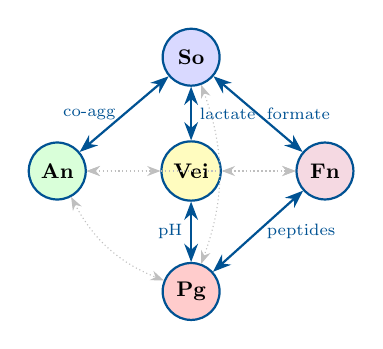
\begin{tikzpicture}[scale=0.85, every node/.style={transform shape},
          species/.style={circle, draw=ikm, thick, minimum size=0.85cm,
                         font=\small\bfseries},
          edge/.style={<->, thick, >=Stealth, ikm},
          weakedge/.style={<->, thin, gray!50, >=Stealth, densely dotted}
      ]
        \node[species, fill=blue!15] (so)  at (0,   2.4) {So};
        \node[species, fill=green!15](an)  at (-2.0, 0.7) {An};
        \node[species, fill=yellow!25](vei) at (0,   0.7) {Vei};
        \node[species, fill=purple!15](fn)  at (2.0, 0.7) {Fn};
        \node[species, fill=red!20]  (pg)  at (0,  -1.1) {Pg};
        \draw[edge] (so) -- (an) node[midway,left,font=\scriptsize] {co-agg};
        \draw[edge] (so) -- (vei) node[midway,right,font=\scriptsize] {lactate};
        \draw[edge] (so) -- (fn) node[midway,right,font=\scriptsize] {formate};
        \draw[edge] (vei) -- (pg) node[midway,left,font=\scriptsize] {pH};
        \draw[edge] (fn)  -- (pg) node[midway,right,font=\scriptsize] {peptides};
        \draw[weakedge] (an) -- (vei);
        \draw[weakedge] (an) -- (fn);
        \draw[weakedge] (vei) -- (fn);
        \draw[weakedge] (so)  to[bend left=20]  (pg);
        \draw[weakedge] (an)  to[bend right=20] (pg);
      \end{tikzpicture}
      \vspace{3pt}
      {\scriptsize \textcolor{ikm}{$\longleftrightarrow$} Confirmed pathway\quad
       \textcolor{gray}{$\cdots$} Free parameter}
  \end{columns}
\end{frame}

% =============================================================================
\section{Mathematical Model}
% =============================================================================

% ─── 2.1 Free energy & variational principle ─────────────────────────────────
\begin{frame}[t]{Free Energy \& Extended Hamilton Principle}
  \small
  \begin{columns}[T]
    \column{0.50\textwidth}
      \textbf{State} (per material point):
      \begin{itemize}
        \item $\phi_i \in (0,1)$: volume fraction, species $i=1\ldots5$
        \item $\psi_i \in (0,1)$: viability fraction
        \item $\bar{\phi}_i := \phi_i\psi_i$: living fraction
        \item $\phi_0$: void / fluid phase
        \item $\gamma$: Lagrange multiplier (volume constraint)
      \end{itemize}
      \vspace{4pt}
      \textbf{Extended Hamilton principle} (Junker \& Balzani 2021):
      \[
        \mathcal{H} = \int_\tau\!\bigl(\mathcal{G} + \mathcal{C} + \mathcal{D}\bigr)\,\mathrm{d}t
        \;\to\; \mathrm{stat}_{\boldsymbol{\xi},\gamma}
      \]
      \vspace{2pt}
      $\mathcal{G}$: free energy\quad $\mathcal{C}$: constraint\quad $\mathcal{D}$: dissipation
    \column{0.48\textwidth}
      \textbf{Free energy density} ($\alpha^*\!=0$, no antibiotics):
      \[
        \Psi = -\tfrac{1}{2}\,c^*\,\bar{\bphi}^{\top}\!\mathbf{A}\,\bar{\bphi}
      \]
      \vspace{2pt}
      \textbf{Dissipation potential} (Klempt et al.\ 2024):
      \[
        \mathcal{D}
        = \tfrac{1}{2}\dot{\bar{\bphi}}^{\top}\!\boldsymbol{\eta}\,\dot{\bar{\bphi}}
        + \tfrac{1}{2}\dot{\bphi}^{\top}\!\boldsymbol{\eta}\,\dot{\bphi}
      \]
      where $\dot{\bar\phi}_i = \dot\phi_i\psi_i + \phi_i\dot\psi_i$,\;
      $\boldsymbol{\eta}=\mathrm{diag}(\eta_i)$, $\eta_i=1$\\[4pt]
      Volume constraint:
      $\displaystyle\mathcal{C}=\gamma\Bigl(\sum_{l=0}^{n}\phi_l - 1\Bigr)$\\[4pt]
      {\scriptsize Barrier $\Psi_{\mathrm{bar}} = K_p/[\phi_i^2(1-\phi_i)^2]$ added numerically\\to enforce $\phi_i,\psi_i\in(0,1)$; omitted from equations for clarity.}
  \end{columns}
\end{frame}

% ─── 2.2 ODE system ──────────────────────────────────────────────────────────
\begin{frame}[t]{Governing ODE System (Euler--Lagrange)}
  \small
  Evaluating $\delta\mathcal{H}=0$ gives coupled equations ($\alpha^*=0$):
  \vspace{2pt}

  \textbf{Volume fraction} $\phi_i$, $i=1,\dots,5$:
  \[
    \boxed{
      0 = -c^*\psi_i\bigl(\mathbf{A}\bar{\bphi}\bigr)_i
      + \eta_i\bigl(\dot\phi_i\psi_i^2 + \bar\phi_i\dot\psi_i + \dot\phi_i\bigr)
      + \gamma
    }
  \]
  \vspace{2pt}
  \textbf{Viability fraction} $\psi_i$:
  \[
    \boxed{
      0 = -c^*\phi_i\bigl(\mathbf{A}\bar{\bphi}\bigr)_i
      + \eta_i\bigl(\dot\psi_i\phi_i^2 + \bar\phi_i\dot\phi_i\bigr)
      + \gamma
    }
  \]
  \vspace{2pt}
  \textbf{Void fraction \& volume constraint:}
  \[
    0 = \gamma + \dot\phi_0,
    \qquad
    0 = \sum_{l=0}^{5}\phi_l - 1
  \]
  \vspace{1pt}
  \begin{columns}[T]
    \column{0.50\textwidth}
      \begin{block}{Interaction term}
        $\bigl(\mathbf{A}\bar{\bphi}\bigr)_i = \displaystyle\sum_{j=1}^{5}A_{ij}\phi_j\psi_j$\\[3pt]
        $A_{ij}=A_{ji}$ (variational symmetry)\\
        $A_{ij}>0$ cooperative; $A_{ij}<0$ competitive
      \end{block}
    \column{0.46\textwidth}
      \begin{block}{Fixed parameters}
        $c^*=25$: nutrient scaling\\
        $\eta_i=1$: viscosity (all species)\\
        $\Delta t=10^{-4}$, $N_t=2500$ steps\\
        $K_p = \eta_i\times10^{-4}$ (barrier)
      \end{block}
  \end{columns}
\end{frame}

% ─── 2.3 Interaction matrix ───────────────────────────────────────────────────
\begin{frame}[t]{Interaction Matrix \& Parameter Space}
  \small
  \begin{columns}[T]
    \column{0.54\textwidth}
      \begin{block}{Symmetric interaction matrix $\mathbf{A}$}
        \[
          \mathbf{A}\in\mathbb{R}^{5\times5},\quad A_{ij}=A_{ji}
          \quad\Rightarrow\quad 15 \text{ independent entries}
        \]
        \vspace{2pt}
        \[
          \mathbf{A}=\begin{pmatrix}
            a_{11} & a_{12} & a_{13} & a_{14} & a_{15}\\
                   & a_{22} & a_{23} & a_{24} & a_{25}\\
                   &        & a_{33} & a_{34} & a_{35}\\
                   &        &        & a_{44} & a_{45}\\
                   &        &        &        & a_{55}
          \end{pmatrix}
        \]
        \vspace{2pt}
        \textbf{Diagonal} $a_{ii}>0$: self-facilitated growth\\
        \textbf{Off-diagonal} $a_{ij}>0$/$<0$: mutualism / competition
      \end{block}
    \column{0.44\textwidth}
      \begin{block}{15 free parameters $\btheta$}
        \[
          \btheta = \bigl(a_{ij}\bigr)_{1\le i\le j\le 5}\in\mathbb{R}^{15}
        \]
        \vspace{2pt}
        Symmetry $A_{ij}=A_{ji}$ is enforced\\
        by the variational structure\\[6pt]
        \textbf{Goal}: infer all 15 parameters\\
        from 4-condition time-series data\\
        \emph{without a priori locking}
      \end{block}
      \vspace{4pt}
      \begin{alertblock}{$\btheta\in\mathbb{R}^{15}$ fully free}
        Biological sparsity (Pg$\approx$0 in\\
        commensal) emerges from data.
      \end{alertblock}
  \end{columns}
\end{frame}

% =============================================================================
\section{Bayesian Inference Framework}
% =============================================================================

\begin{frame}[t]{TMCMC: Transitional Markov Chain Monte Carlo}
  \small
  \begin{columns}[T]
    \column{0.52\textwidth}
      \textbf{Goal}: compute posterior
      \[
        p(\btheta\mid\mathbf{y}_{\mathrm{obs}})
        \propto p(\mathbf{y}_{\mathrm{obs}}\mid\btheta)\,p(\btheta)
      \]
      \textbf{TMCMC} (Ching \& Chen 2007):
      \[
        p_m(\btheta) \propto p(\mathbf{y}_{\mathrm{obs}}\mid\btheta)^{\beta_m}\,p(\btheta),
        \quad 0=\beta_0 < \cdots < \beta_M = 1
      \]
      At each stage $m$:
      \begin{enumerate}
        \item \textbf{Resample} $N_p$ particles $\propto w_j^{(m)}$
        \item \textbf{Estimate} weighted covariance $\hat{\boldsymbol{\Sigma}}^{(m)}$
        \item \textbf{Mutate} via MH with $\mathcal{N}(\btheta_j, \gamma^2\hat{\boldsymbol{\Sigma}}^{(m)})$
      \end{enumerate}
      \vspace{4pt}
      By-product: log-evidence estimate $\ln\hat{Z}$
    \column{0.46\textwidth}
      \begin{block}{Likelihood}
        \[
          \ln p(\mathbf{y}\mid\btheta) =
          -\sum_{k,i}\frac{(y_{i,k}-\hat{y}_{i,k}(\btheta))^2}{2\sigma_i^2}
        \]
        $\sigma_i$: species-specific replicate noise ($\approx 0.05$--$0.20$)
      \end{block}
      \vspace{4pt}
      \begin{block}{Prior}
        Independent uniform: $p(\btheta)=\prod_{k=0}^{14}\frac{1}{u_k-l_k}$\\[4pt]
        Bounds iteratively narrowed after Phase~1:\\
        $[q_{0.01}-1.5\sigma,\;q_{0.99}+1.5\sigma]$
      \end{block}
  \end{columns}
\end{frame}

\begin{frame}[t]{Two-Phase Estimation Strategy}
  \centering
  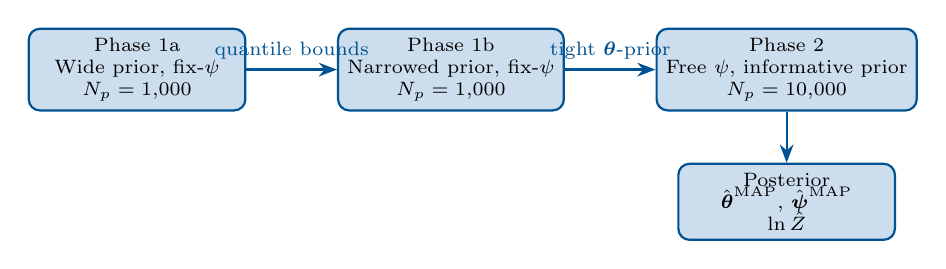
\begin{tikzpicture}[
    node distance=0.65cm and 1.15cm,
    box/.style={rectangle, rounded corners, draw=ikm, thick, fill=ikmlight,
                minimum width=2.75cm, minimum height=0.72cm, align=center, font=\scriptsize},
    arrow/.style={->, thick, >=Stealth, color=ikm}
  ]
    \node[box] (p1a) {Phase 1a\\Wide prior, fix-$\psi$\\$N_p=1{,}000$};
    \node[box, right=of p1a] (p1b) {Phase 1b\\Narrowed prior, fix-$\psi$\\$N_p=1{,}000$};
    \node[box, right=of p1b] (p2)  {Phase 2\\Free $\psi$, informative prior\\$N_p=10{,}000$};
    \node[box, below=of p2]  (out) {Posterior\\$\hat{\btheta}^{\mathrm{MAP}}$, $\hat{\bpsi}^{\mathrm{MAP}}$\\$\ln\hat{Z}$};

    \draw[arrow] (p1a) -- node[above,font=\scriptsize]{quantile bounds} (p1b);
    \draw[arrow] (p1b) -- node[above,font=\scriptsize]{tight $\btheta$-prior} (p2);
    \draw[arrow] (p2)  -- (out);
  \end{tikzpicture}
  \vspace{0.25cm}
  \begin{columns}[T]
    \column{0.49\textwidth}
      \small
      \begin{block}{Phase 1 (fix-$\psi$)}
        \begin{itemize}
          \item Robust identification of $\mathbf{A}$
          \item Reduced posterior multimodality
        \end{itemize}
      \end{block}
    \column{0.49\textwidth}
      \small
      \begin{block}{Phase 2 (free $\psi$)}
        \begin{itemize}
          \item Joint posterior for $(\mathbf{A},\bpsi)$
          \item Phase~1 posterior as informative $\btheta$-prior
        \end{itemize}
      \end{block}
  \end{columns}
\end{frame}

\begin{frame}[t]{Phase 1 / Phase 2 Details}
  \small
  \begin{columns}[T]
    \column{0.49\textwidth}
      \begin{block}{Phase 1 — Fix-$\psi$}
        \begin{itemize}
          \item Fix $\psi_i(t_k) = \psi_i^{\mathrm{exp}}(t_k)$
          \item Eliminates $\psi$-related posterior modes
          \item Halves ODE Jacobian dimension
          \item Identifies $\mathbf{A}$ rapidly and robustly
        \end{itemize}
      \end{block}
    \column{0.49\textwidth}
      \begin{block}{Phase 2 — Free $\psi$}
        \begin{itemize}
          \item Release $\psi_i$ as free variables
          \item Viability data as \emph{soft constraint}:\\
                $\ln\mathcal{L} +{=} -\sum(\psi_i-\psi_i^{\mathrm{exp}})^2/(2\cdot0.1^2)$
          \item Phase~1 posterior as informative $\btheta$-prior
          \item Physically consistent joint posterior
        \end{itemize}
      \end{block}
  \end{columns}
\end{frame}

% =============================================================================
\section{GPU Acceleration}
% =============================================================================

\begin{frame}[t]{GPU-Parallel Forward Model}
  \small
  \begin{columns}[T]
    \column{0.52\textwidth}
      \textbf{Computational bottleneck}:\\
      $\mathcal{O}(10^5)$--$\mathcal{O}(10^6)$ ODE solves per run\\
      ($N_p=10{,}000$ particles $\times$ $K=20$ MH steps $\times$ $M\approx5$ stages)
      \vspace{8pt}

      \textbf{JAX implementation}:
      \begin{itemize}
        \item Implicit Euler--Newton solver compiled via \texttt{jax.jit}
        \item All $N_p$ particles evaluated simultaneously via \texttt{jax.vmap}
        \item Single fused XLA kernel (no Python overhead)
      \end{itemize}
      \vspace{6pt}
      \begin{block}{Adaptive $\gamma$ scaling}
        Initialised $\gamma^2 = 2.38^2/15$ (Roberts et al.\ optimal)\\
        Online: halve if $\bar{\alpha}<5\%$; increase $50\%$ if $\bar{\alpha}>40\%$
      \end{block}
    \column{0.46\textwidth}
      \centering
      \begin{tabular}{@{}lrrr@{}}
        \toprule
        \textbf{Metric} & \textbf{CPU} & \textbf{GPU} & \textbf{Speedup}\\
        \midrule
        \multicolumn{4}{@{}l}{\textit{Matched benchmark ($N_p=500$, DH):}}\\
        \quad Per stage  & 2\,400\,s & 14\,s  & $170\times$\\
        \quad Total      & 21\,600\,s & 147\,s & $\mathbf{200\times}$\\
        \midrule
        \multicolumn{4}{@{}l}{\textit{Production ($N_p=10{,}000$):}}\\
        \quad Per cond.  & $\sim$120\,h & 1.7--2.6\,h & $\sim$50$\times$\\
        \quad 4 cond.    & $\sim$480\,h & 8\,h  & $\sim$60$\times$\\
        \bottomrule
      \end{tabular}
      \vspace{8pt}

      \textbf{Hardware}: NVIDIA RTX\,4090\\
      \textbf{CPU baseline}: 12-core Intel\\[4pt]
      \textcolor{red!70!black}{\textbf{$\sim$200$\times$ speedup}} at matched settings\\
      Production runs feasible in $\sim$2\,h/condition
  \end{columns}
\end{frame}

% =============================================================================
\section{Results}
% =============================================================================

\begin{frame}[t]{Quantitative Fit Metrics}
  \small
  \begin{columns}[T]
    \column{0.56\textwidth}
      \centering
      \vspace{2pt}
      \begin{tabular}{@{}l
          r r
          r r r@{}}
        \toprule
        & \multicolumn{2}{c}{\textbf{Phase 1}} & \multicolumn{3}{c}{\textbf{Phase 2 (final)}}\\
        \cmidrule(lr){2-3}\cmidrule(lr){4-6}
        \textbf{Cond.} & RMSE & MAE & RMSE & MAE & $\ln\hat{Z}$\\
        \midrule
        CS & 0.119 & 0.077 & 0.119 & 0.075 & $-3.3$\\
        CH & 0.071 & 0.053 & 0.104 & 0.088 & $-8.5$\\
        DS & \textbf{0.020} & \textbf{0.025} & \textbf{0.033} & \textbf{0.024} & $\mathbf{-2.8}$\\
        DH & 0.067 & 0.045 & 0.087 & 0.060 & $-11.9$\\
        \bottomrule
      \end{tabular}
      \vspace{4pt}
      {\scriptsize Phase 1: fix-$\psi$, $N_p=1{,}000$\quad Phase 2: free $\psi$, $N_p=10{,}000$}
    \column{0.42\textwidth}
      \vspace{2pt}
      \begin{block}{Key observations}
        \begin{itemize}\setlength{\itemsep}{3pt}
          \item DS: lowest RMSE (\hlnum{0.033}) — best identifiability
          \item Phase~2 $\Delta$RMSE $\leq 0.03$ — Phase~1 robust
          \item DH Pg trajectory: gingipain $r=0.90$
        \end{itemize}
      \end{block}
      \vspace{4pt}
      \begin{block}{Convergence}
        \begin{itemize}\setlength{\itemsep}{3pt}
          \item $M=4$--$7$ stages, $\bar\alpha=7$--$13\%$
          \item $\mathrm{ESS}=N_p$ at final stage
          \item Gelman--Rubin $\hat{R}<1.1$ (all params)
        \end{itemize}
      \end{block}
  \end{columns}
\end{frame}

\begin{frame}[plain]{Posterior Predictive Fits}
  \vspace{-0.1cm}
  \centering
  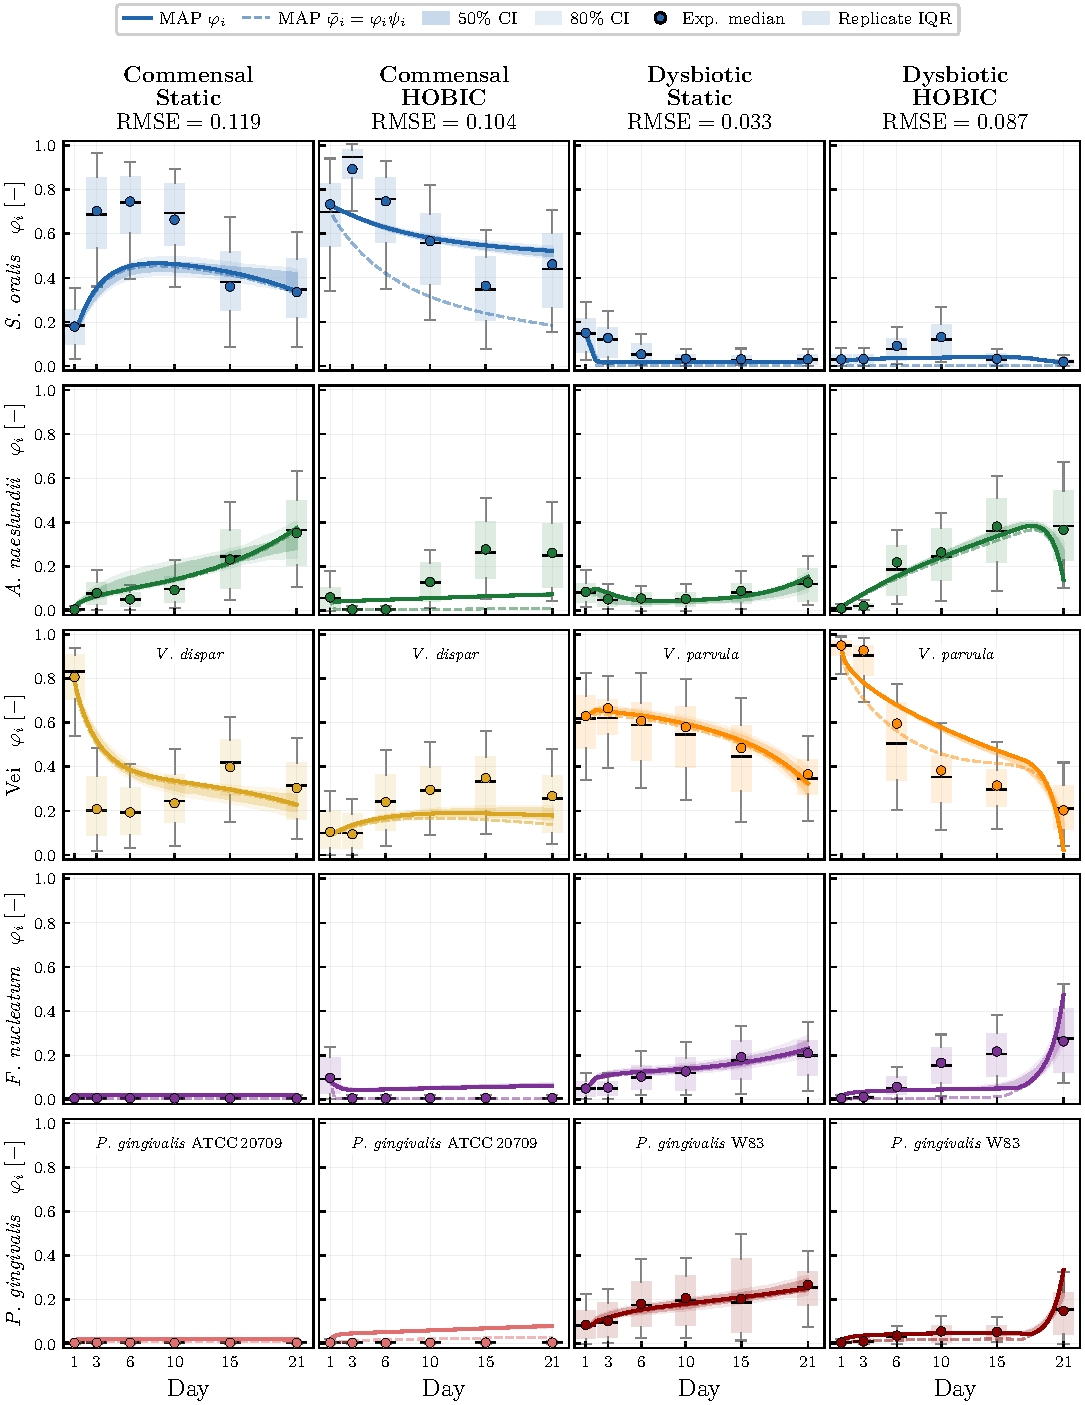
\includegraphics[height=0.80\textheight,keepaspectratio]{figures/paper_fig2_phi_transposed.pdf}
  \par\vspace{3pt}
  {\color{gray}\rule{0.9\textwidth}{0.3pt}}\par\vspace{2pt}
  {\scriptsize
   Columns: CS\;CH\;DS\;DH (increasing dysbiotic severity)\enspace
   Rows: So, An, Vei, Fn, Pg\enspace
   Solid: MAP $\phi_i$\enspace Dashed: $\bar\phi_i=\phi_i\psi_i$\enspace
   Shaded: 50\%/80\% CI (100 samples)}
\end{frame}

\begin{frame}[t]{Inferred Interaction Matrices}
  \centering
  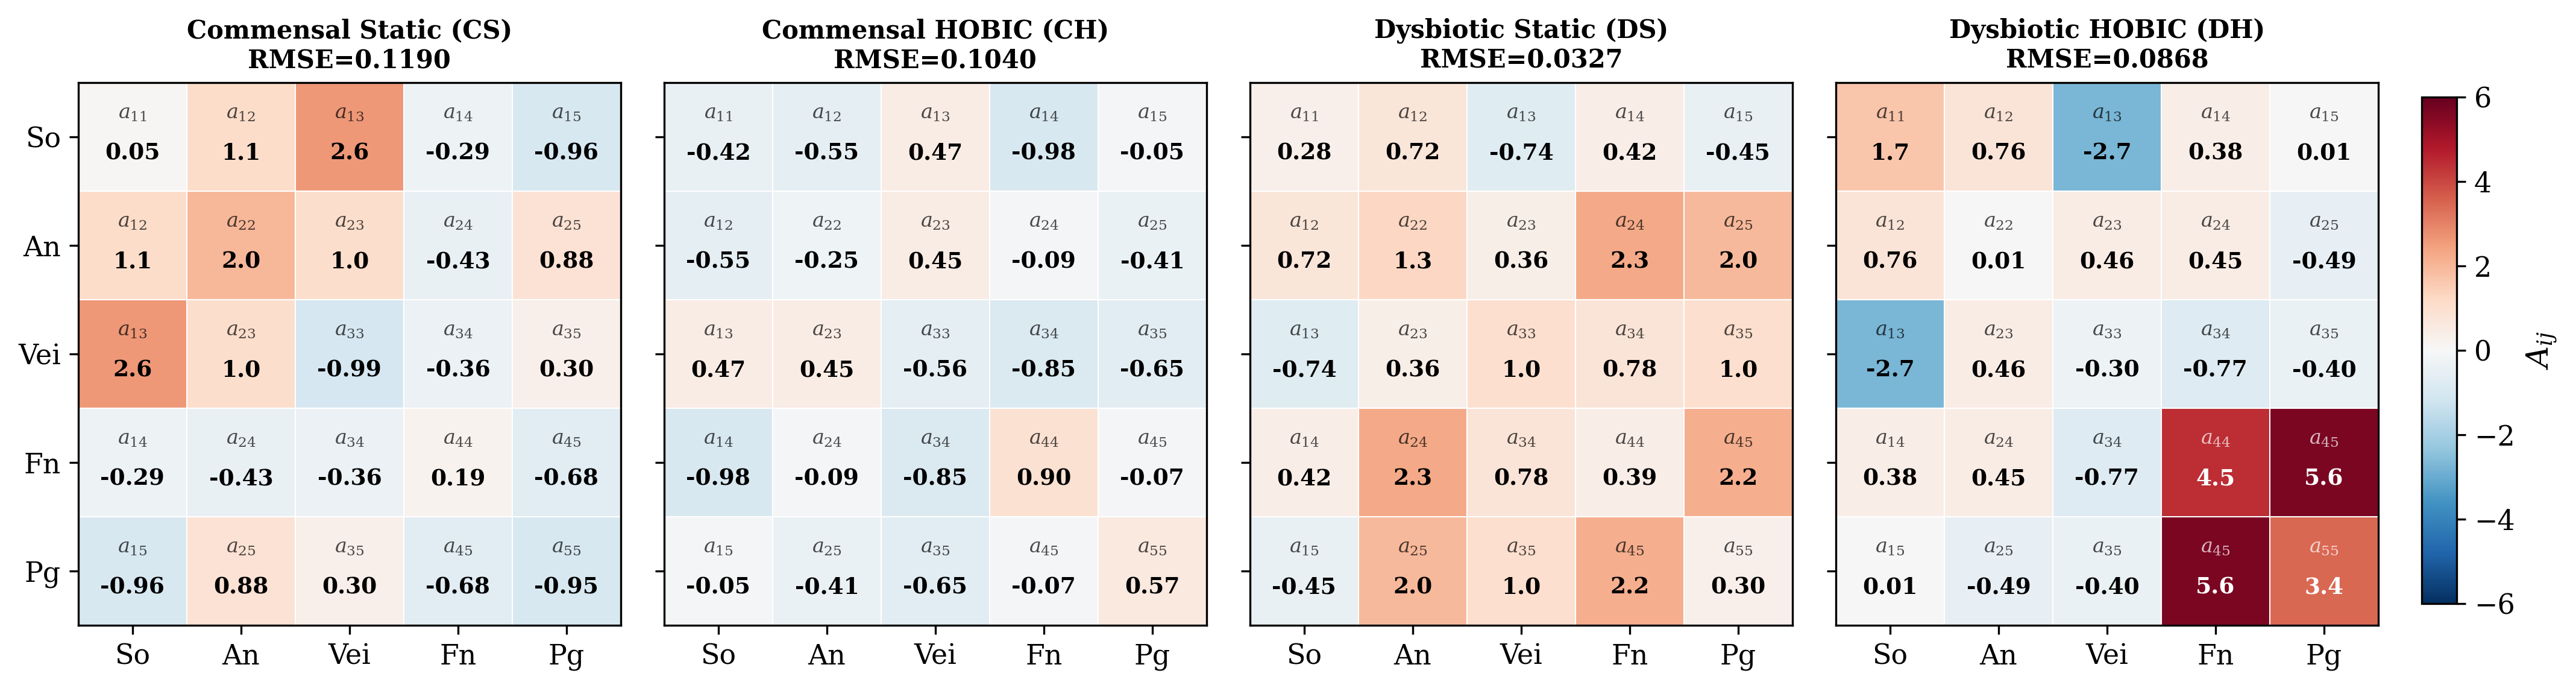
\includegraphics[width=\textwidth,height=0.58\textheight,keepaspectratio]{figures/heatmap_A_4cond.pdf}
  \par\vspace{3pt}
  \begin{columns}[T]
    \column{0.48\textwidth}
      \small\textbf{Commensal (CS, CH):}
      \begin{itemize}\setlength{\itemsep}{2pt}
        \item So--An and So--Vei blocks dominant
        \item Fn, Pg rows near \textbf{zero} (emergent)
      \end{itemize}
    \column{0.48\textwidth}
      \small\textbf{Dysbiotic (DS, DH):}
      \begin{itemize}\setlength{\itemsep}{2pt}
        \item Strong Vei$\to$Pg + Fn$\to$Pg
        \item \hlnum{$\hat{a}_{45}^{\mathrm{DH}}=5.63$}: pathogen surge
      \end{itemize}
  \end{columns}
\end{frame}

\begin{frame}[plain]{Posterior Parameter Distributions}
  \vspace{-0.1cm}
  \centering
  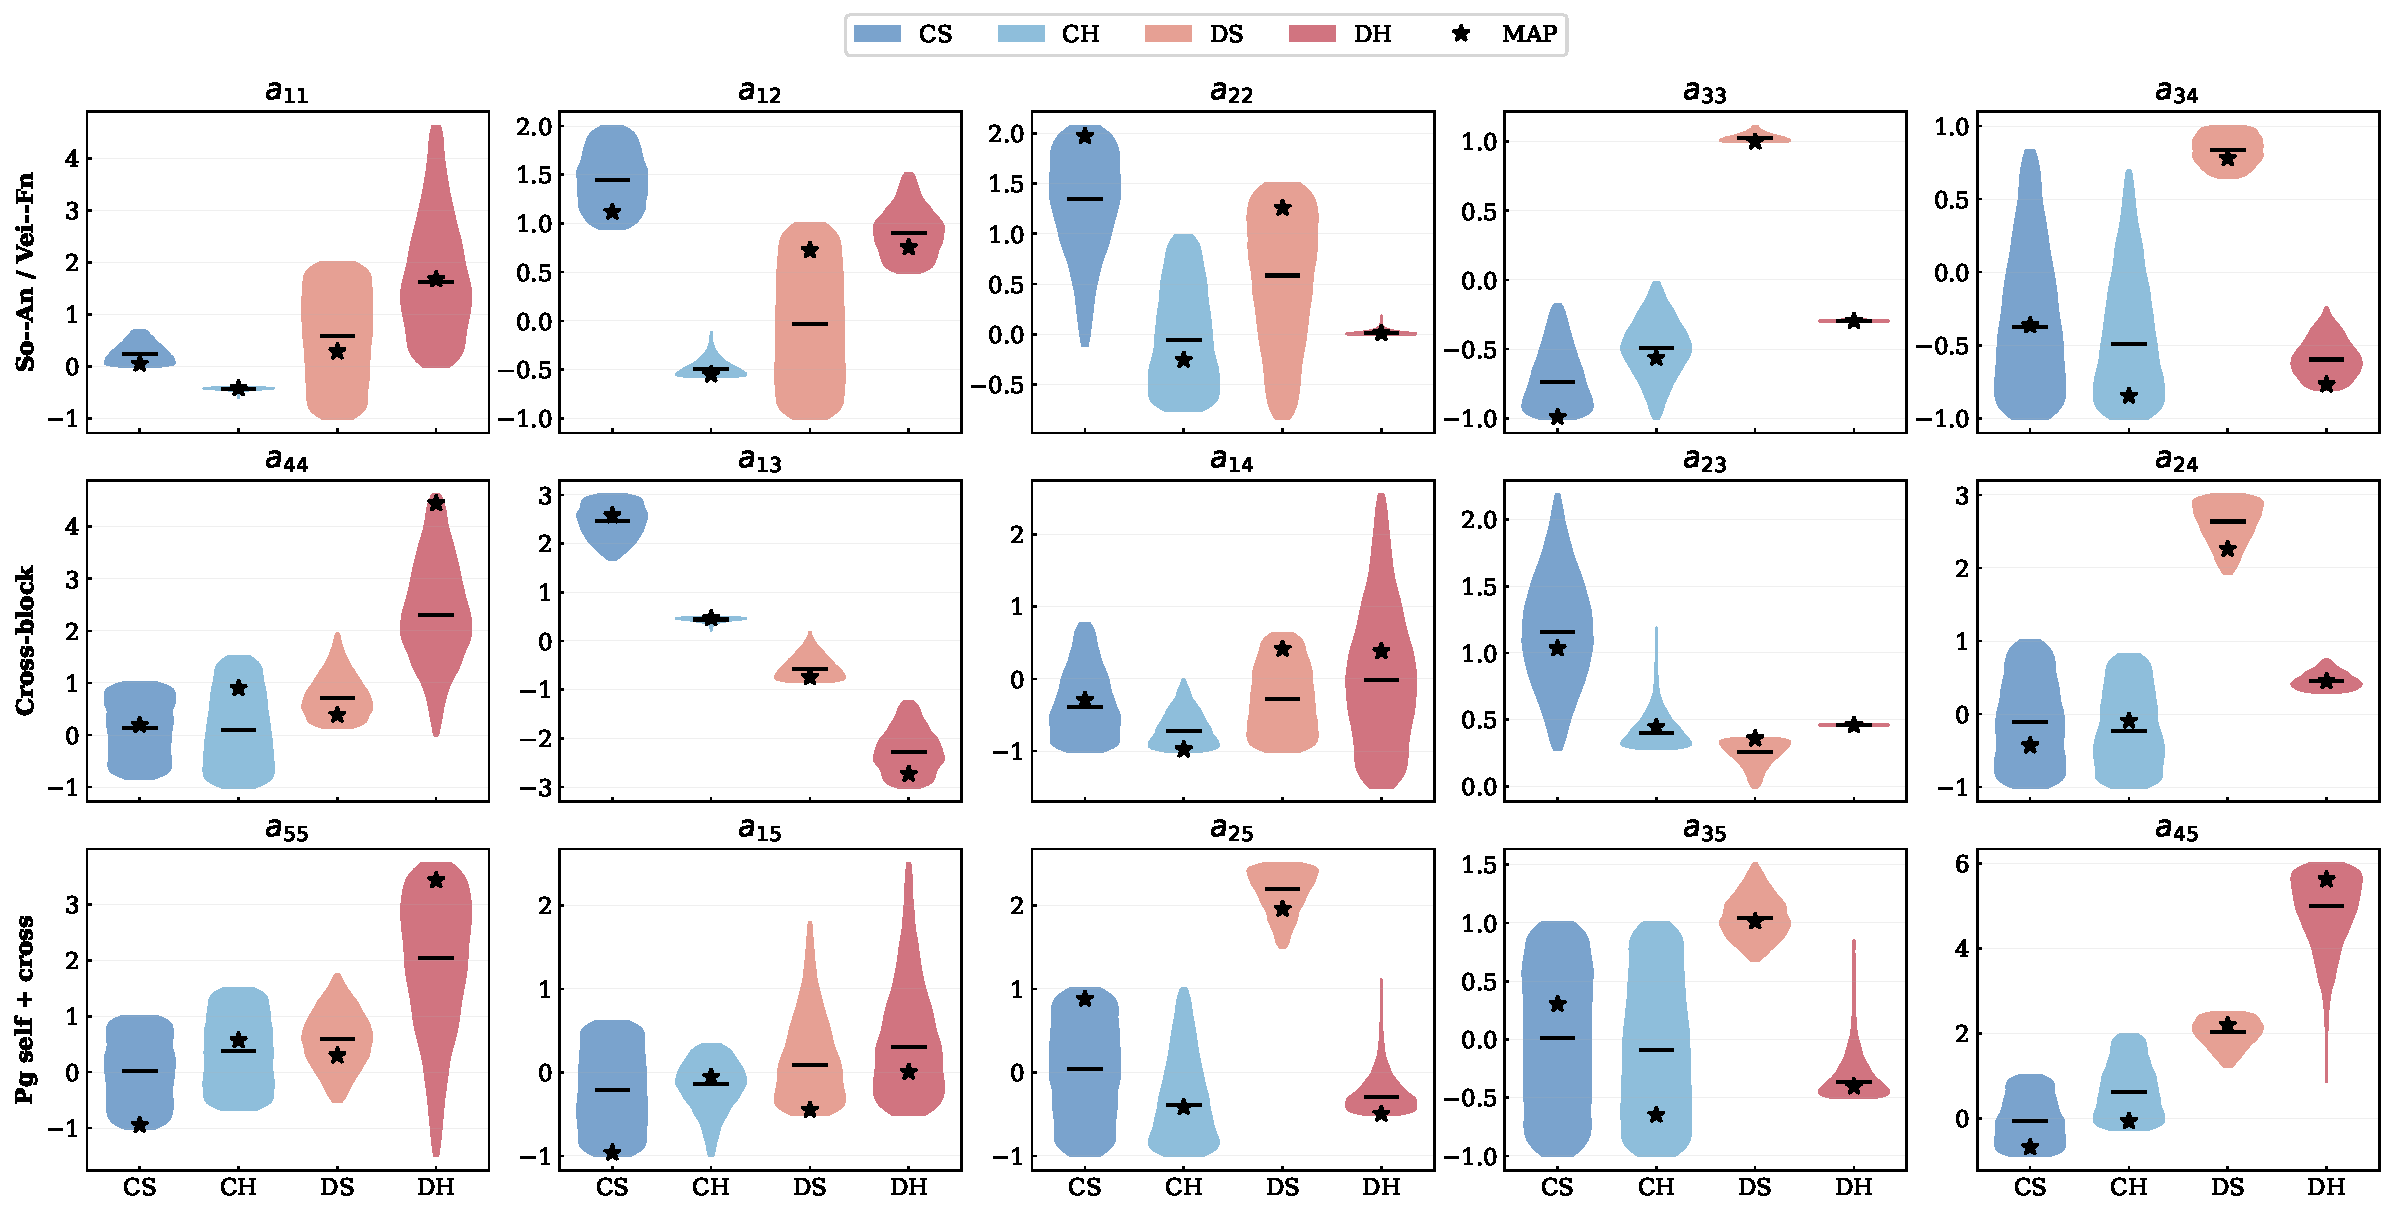
\includegraphics[height=0.80\textheight,keepaspectratio]{figures/paper_posterior_violin.pdf}
  \par\vspace{3pt}
  {\color{gray}\rule{0.9\textwidth}{0.3pt}}\par\vspace{2pt}
  {\scriptsize All 15 $\mathbf{A}$-entries, Phase~2 ($N_p=10{,}000$)\enspace
   Stars: MAP\enspace
   CS/CH: Pg params ($a_{15},a_{25},a_{35},a_{45},a_{55}$) concentrate near zero
   \emph{without a priori locking}}
\end{frame}

\begin{frame}[t]{Phase 1 vs Phase 2 Consistency}
  \centering
  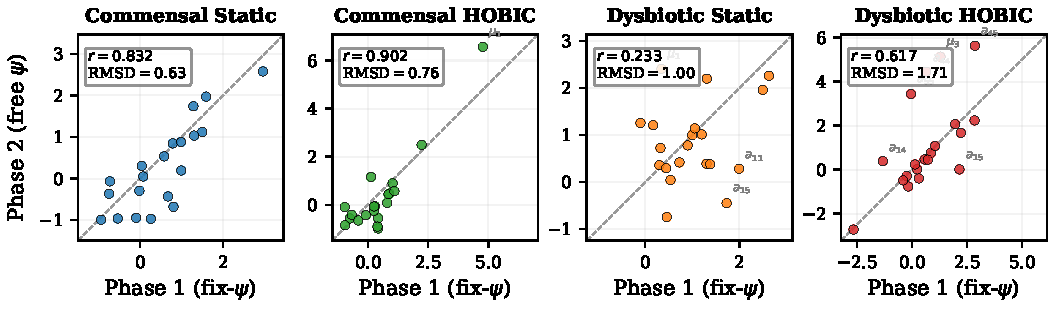
\includegraphics[width=\textwidth,height=0.58\textheight,keepaspectratio]{figures/phase1_vs_phase2_map.pdf}
  \par\vspace{3pt}
  \begin{columns}[T]
    \column{0.48\textwidth}
      \small\textbf{Commensal (CS, CH):}
      \begin{itemize}\setlength{\itemsep}{1pt}
        \item CS: $r=0.87$, CH: $r=0.68$
        \item fix-$\psi$ is a valid approximation
      \end{itemize}
    \column{0.48\textwidth}
      \small\textbf{Dysbiotic (DS, DH):}
      \begin{itemize}\setlength{\itemsep}{1pt}
        \item DS: $r=0.42$, DH: $r=0.62$
        \item Shift in $a_{55}$, $a_{15}$, $a_{45}$
        \item Phase~2 essential for dysbiosis
      \end{itemize}
  \end{columns}
\end{frame}

\begin{frame}[t]{Cross-Condition Transferability}
  \small
  \begin{columns}[T]
    \column{0.46\textwidth}
      \centering
      \vspace{4pt}
      \begin{tabular}{@{}l cccc@{}}
        \toprule
        \small Source $\to$ Target & CS & CH & DS & DH \\
        \midrule
        CS & \textit{.273} & \textbf{.135} & \textbf{.111} & .244 \\
        CH & .229 & \textit{.168} & \textbf{.127} & .233 \\
        DS & .273 & .130 & \textit{.062} & .252 \\
        DH & .301 & .129 & \textbf{.044} & \textit{.262} \\
        \bottomrule
      \end{tabular}
      \vspace{3pt}
      {\scriptsize \textit{Italic}: self-prediction.\quad
       \textbf{Bold}: transfer beats self.}
    \column{0.52\textwidth}
      \textbf{Findings:}
      \begin{itemize}\setlength{\itemsep}{3pt}
        \item \textbf{Within-state} transfer works well:\\
              DH$\to$DS = \hlnum{0.044} beats DS self (0.062)\\
              CS$\to$CH = 0.135 vs.\ CH self 0.168
        \item \textbf{Cross-state} degrades sharply:\\
              DS$\to$CS = 0.273, CS$\to$DH = 0.244
        \item Dysbiotic backbone: $\rho_{\mathrm{DH}-DS}=+0.40$
        \item Cross-state anticorr.: $\rho_{\mathrm{DH}-CS}=-0.49$
      \end{itemize}
      \vspace{5pt}
      \begin{alertblock}{}
        Health$\to$Disease: \textbf{topological reorganisation},\\
        not mere parameter rescaling
      \end{alertblock}
  \end{columns}
\end{frame}

% =============================================================================
\section{Validation \& Discussion}
% =============================================================================

\begin{frame}[t]{Independent Validation}
  \small
  \begin{block}{\small 4 held-out measurements from Heine et al.\ (2025) — \emph{not} used in calibration}
  \end{block}
  \vspace{4pt}
  \begin{columns}[T]
    \column{0.49\textwidth}
      \textbf{1.\ pH prediction}
      \begin{itemize}\setlength{\itemsep}{2pt}
        \item $R^2=\hlnum{0.71}$, $r=\hlnum{0.84}$ ($N=12$)
        \item pH $= 6.95 - 0.74\,\phi_{\mathrm{So}} - 0.48\,\phi_{\mathrm{Vei}}$
        \item Negative So: lactate-driven acidification
      \end{itemize}
      \vspace{6pt}
      \textbf{2.\ Gingipain--Pg correlation}
      \begin{itemize}\setlength{\itemsep}{2pt}
        \item $r=\hlnum{0.90}$ (5 time points, DH)
        \item Both show delayed onset at Day~15--21
      \end{itemize}
    \column{0.49\textwidth}
      \textbf{3.\ Metabolic sign consistency}
      \begin{itemize}\setlength{\itemsep}{2pt}
        \item MAP $A_{12}=+0.76$ (An$\to$Vei):\\
              lactate/succinate cross-feeding \checkmark
        \item MAP $A_{13}=-2.73$ (So$\to$Vei):\\
              niche competition dominates
      \end{itemize}
      \vspace{6pt}
      \textbf{4.\ Growth rate parity}
      \begin{itemize}\setlength{\itemsep}{2pt}
        \item Commensal: 1.68\,h\; vs.\ Dysbiotic: 1.64\,h
        \item Differences from interactions,\\
              not individual fitness
      \end{itemize}
  \end{columns}
\end{frame}

\begin{frame}[t]{Biological Interpretation}
  \small
  \begin{columns}[T]
    \column{0.48\textwidth}
      \begin{block}{Commensal state (CS, CH)}
        \begin{itemize}
          \item So--An co-aggregation + So--Vei lactate exchange: \textbf{stable mutualistic core}
          \item Fn and Pg entries near zero (emergent sparsity)
          \item HOBIC flow shifts So abundance but preserves community structure
        \end{itemize}
      \end{block}
      \vspace{6pt}
      \begin{block}{Dysbiotic transition}
        \begin{itemize}
          \item Vei$\to$Pg (pH elevation) + Fn$\to$Pg (peptide supply) strongly activated
          \item \textbf{Topological reorganisation}: $\rho_{\mathrm{DH}-CS}=-0.49$
          \item Not recoverable by parameter rescaling
        \end{itemize}
      \end{block}
    \column{0.50\textwidth}
      \begin{block}{Model parsimony (effective dimensionality)}
        $r_i = \sigma_{{\mathrm{post}},i}/\Delta_{\mathrm{prior}}$ ($\Delta_{\mathrm{prior}}=6$)
        \vspace{4pt}
        \begin{itemize}
          \item All 15 params: $r_i < 0.43$ in every condition
          \item DS tightest (mean $r=0.07$)
          \item Even Pg-related in commensal: $r_i\leq0.10$
          \item[$\Rightarrow$] Posterior constrains them near zero,\\
                not prior-dominated
        \end{itemize}
        \vspace{4pt}
        \textcolor{ikm}{\textbf{Full 15-parameter model justified.}}
      \end{block}
  \end{columns}
\end{frame}

\begin{frame}[t]{Fix-$\psi$ Approximation}
  \small
  \begin{columns}[T]
    \column{0.56\textwidth}
      \centering
      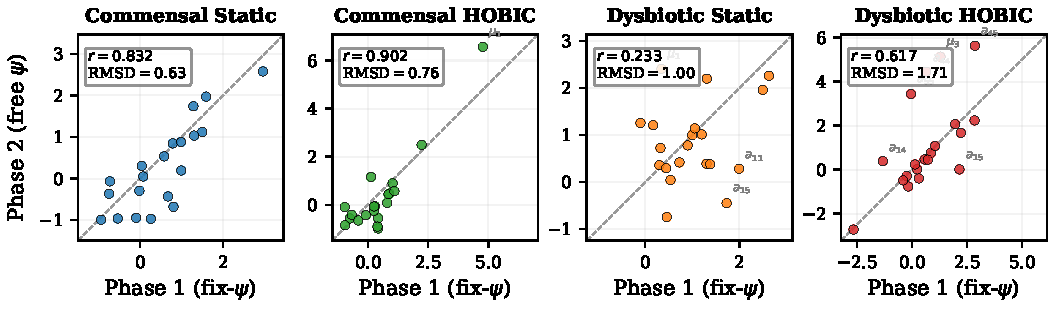
\includegraphics[width=\linewidth,height=0.68\textheight,keepaspectratio]{figures/phase1_vs_phase2_map.pdf}
      \par{\scriptsize Phase 1 vs.\ Phase 2 MAP (15 parameters each)}
    \column{0.42\textwidth}
      \vspace{6pt}
      \textbf{Why fix-$\psi$ works (commensal):}
      \begin{itemize}\setlength{\itemsep}{2pt}
        \item $\psi$--$\mathbf{A}$ coupling weak when Pg $\approx 0$
        \item CS $r=0.87$, CH $r=0.68$
      \end{itemize}
      \vspace{6pt}
      \textbf{Why Phase~2 is essential (dysbiosis):}
      \begin{itemize}\setlength{\itemsep}{2pt}
        \item DS $r=0.42$, DH $r=0.62$
        \item Pg viability feeds back onto $a_{55}$, $a_{45}$
        \item Viability RMSE 0.11--0.39
      \end{itemize}
      \vspace{6pt}
      \begin{alertblock}{Strategy validated}
        Phase~1: reliable $\mathbf{A}$ identification\\
        Phase~2: critical for dysbiotic conditions
      \end{alertblock}
  \end{columns}
\end{frame}

% =============================================================================
\section{Conclusions}
% =============================================================================

\begin{frame}[t]{Conclusions}
  \small
  \begin{columns}[T]
    \column{0.49\textwidth}
      \begin{block}{\raisebox{0pt}[0pt][0pt]{1.\ Two-phase estimation}}
        \begin{itemize}\setlength{\itemsep}{2pt}
          \item Phase~1 (fix-$\psi$): rapid, robust $\mathbf{A}$ identification
          \item Phase~2 (free $\psi$): physically consistent joint posterior
          \item All \hlnum{15} params free — sparsity emerges from data
        \end{itemize}
      \end{block}
      \vspace{5pt}
      \begin{block}{\raisebox{0pt}[0pt][0pt]{2.\ GPU-accelerated TMCMC}}
        \begin{itemize}\setlength{\itemsep}{2pt}
          \item JAX + \texttt{jax.vmap} on NVIDIA RTX\,4090
          \item \hlnum{${\sim}200\times$} speedup at matched settings
          \item Production: $N_p=10{,}000$ in \hlnum{${\sim}2$\,h}/condition
        \end{itemize}
      \end{block}
    \column{0.49\textwidth}
      \begin{block}{\raisebox{0pt}[0pt][0pt]{3.\ Independent validation}}
        \begin{itemize}\setlength{\itemsep}{2pt}
          \item pH: $r=\hlnum{0.84}$ ($N=12$, not used in fit)
          \item Gingipain--Pg: $r=\hlnum{0.90}$ (5 time points)
          \item Metabolic signs consistent
        \end{itemize}
      \end{block}
      \vspace{5pt}
      \begin{block}{\raisebox{0pt}[0pt][0pt]{4.\ Quantitative dysbiosis transition}}
        \begin{itemize}\setlength{\itemsep}{2pt}
          \item Within-state transfer beats self-fit
          \item $\rho_{\mathrm{DH}-CS}=-0.49$: topological reorganisation,\\
                not parameter rescaling
        \end{itemize}
      \end{block}
  \end{columns}
\end{frame}

\begin{frame}[t]{Future Work}
  \small
  \begin{columns}[T]
    \column{0.49\textwidth}
      \begin{block}{Computational extensions}
        \begin{itemize}\setlength{\itemsep}{3pt}
          \item \textbf{DeepONet surrogate}: ${\sim}100\times$ TMCMC speedup
                (12--18\,s vs.\ ${\sim}30$\,min, trained per condition)
          \item \textbf{NUTS/HMC}: gradient-based mutation via
                JAX autodiff ($1.75\times$ acceptance vs.\ RW)
          \item \textbf{Spatial PDE}: 2D Hamilton + nutrient field
                $\to$ spatially resolved DI($x,y$)
        \end{itemize}
      \end{block}
    \column{0.49\textwidth}
      \begin{block}{Biological extensions}
        \begin{itemize}\setlength{\itemsep}{3pt}
          \item \textbf{6-species validation}: Siddiqui et al.\ (2021)
                cpTi biofilm data (21 days, 6 time points)
          \item \textbf{Mechanistic pH model}: Henderson--Hasselbalch
                + lactate production from So/Vei
          \item \textbf{VEM-based FEM}: biofilm conformal mesh
                with Virtual Element Method
        \end{itemize}
      \end{block}
  \end{columns}
  \vspace{8pt}
  \centering
  {\color{ikm}\rule{0.5\textwidth}{0.6pt}}\\[4pt]
  \small\textit{All code and data available upon request.}
\end{frame}

% =============================================================================
\end{document}
